\documentclass[12pt,oneside]{article}\usepackage[utf8]{inputenc}\usepackage[a4paper]{geometry}\usepackage{graphicx,setspace,appendix,mathrsfs,amsmath,amsfonts,array,tabularx,longtable,rotating,caption,mathtools,natbib}\usepackage[english]{babel}\renewcommand{\baselinestretch}{1.25}\bibliographystyle{agsm}\doublespacing\title{Information acquisition in China's college admission mechanisms}\author{Yao Luo}\begin{document}\maketitle

\section{Motivation}
\begin{frame}{Motivation}
Theoretical results tell us:
\vspace{0.5cm}
    \begin{itemize}
        \item Matching literature assume full information. But a few papers show that people need to conduct costly information acquisition to discover their preferences.(Corcoran et al. 2018, Dynarski et al. 2020, Grenet et al. 2019)\\
        \item Market designers should pay attention to the acquisition and flow of information.\\
        \item Follow Azevedo and Loshno (2016) and Immorlica et al (2020), finding regret-free stable matching outcomes is equivalebt to finding market-clearing cutoffs.\\
        \item Information deadlocks. Market-clearing cutoffs $\rightarrow$ budget set $\rightarrow$ preference formation $\rightarrow$ determine cutoffs
    \end{itemize}
\end{frame}

\begin{frame}{Motivation}
Real mechanism implementations:
\vspace{0.5cm}
    \begin{itemize}
        \item Achieve approximately regret-free stable outcomes by providing external historical data with respect to perturbed capacities: Australia\\
        \item In 2023 Australia has 62,846 applicants, while China has 12,910,000 applicants. \\
        \item Parallel admission mechanism (PA) - Direct serial dictatorship with length restriction of the rank-ordered list (ROL)\\
        \item Inner Mongolia dynamic admission mechanism (IM) - Sequential serial dictatorship + sequential moves by groups instead of individuals + time constraints\\
        \item In 2025 Inner Mongolia will give up IM and use PA. IM began in 2007. 
    \end{itemize}
\end{frame}

\begin{frame}{Motivation}
    \begin{itemize}
        \item Both PA and IM provides historical cutoff scores, but IM offers additional information regarding matching outcomes.\\
        \item Theoretically and experimentally, a sequential serial dictatorship mechanism leads to higher student welfare than a direct serial dictatorship mechanism. (Hakimov et all, 2023)

    \end{itemize}
\end{frame}
\begin{frame}{Motivation}
\begin{figure}[h!]
\centering
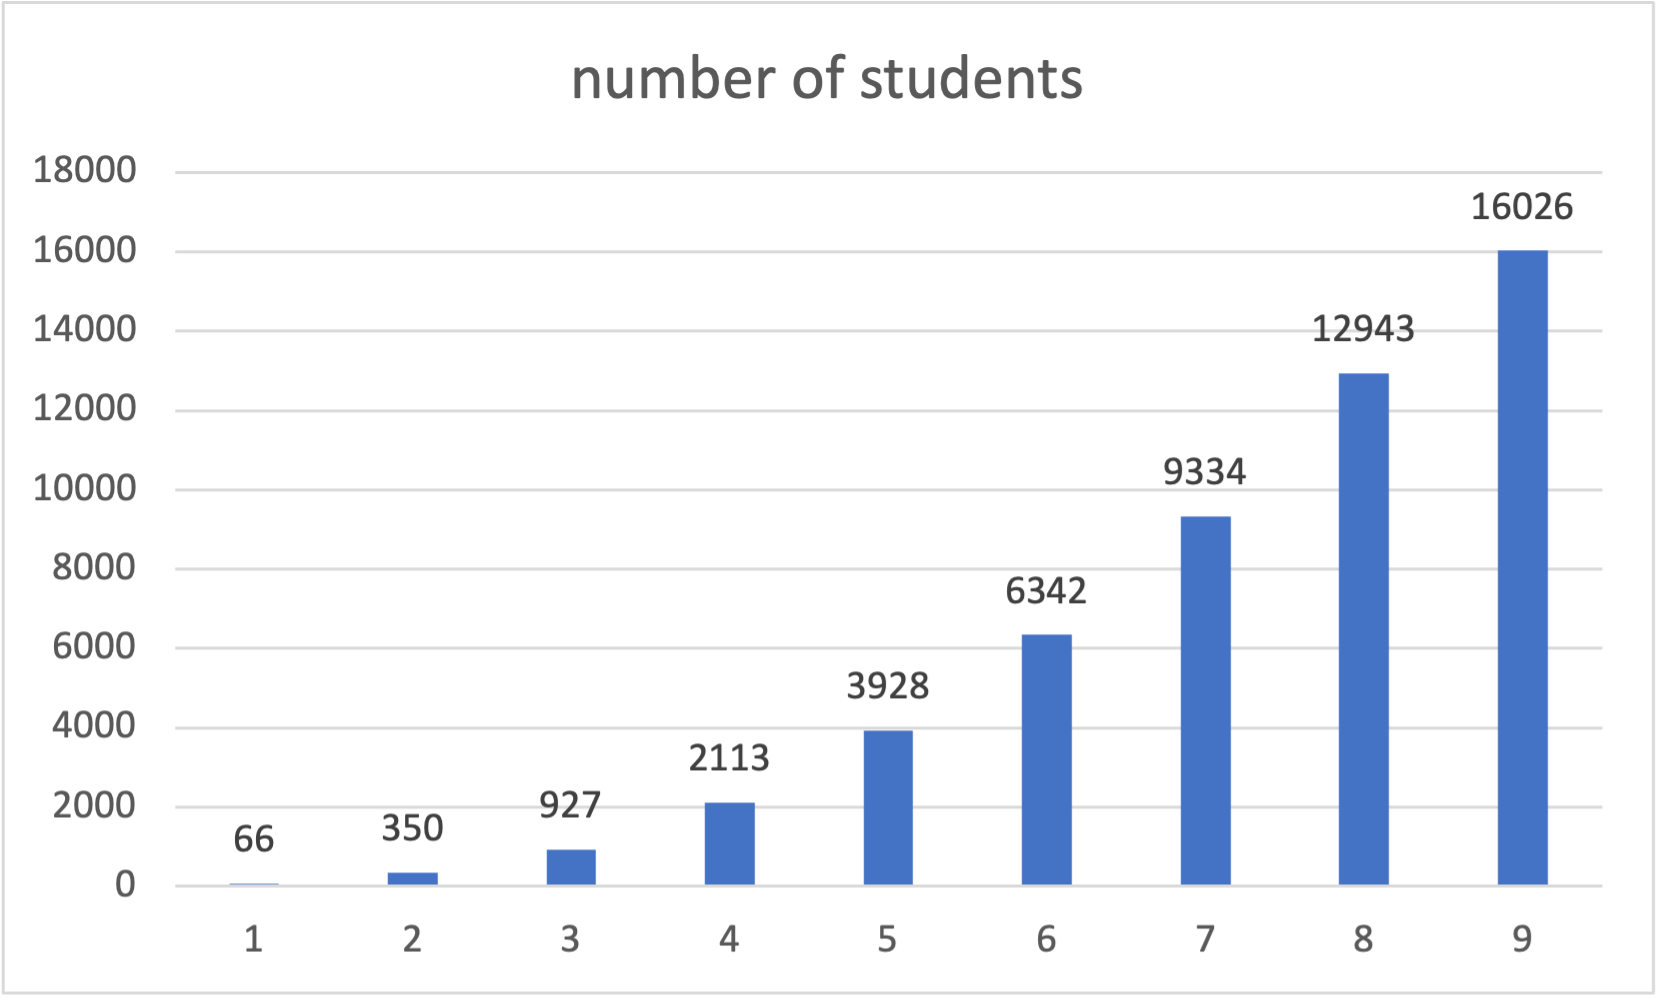
\includegraphics[width=0.8\textwidth]{1.png}
\end{figure}
\end{frame}




\section{Research question}
\begin{frame}{Research question}
    \begin{itemize}
    	\item First guess IM better than PA since IM provides additional information. Seems counterituitive.\\
    	\item Maybe the time constraints in IM (one hour per group) make the price discovery process too costly. Maybe information communication in IM is not effective. Maybe the additional information is too noisy and detriment students' welfare instead. Or maybe IM is indeed better than PA and the policy change is purely of political intention. 
        \item Are there better ways to communicate information to students to improve matching outcomes of IM? \\
    \end{itemize}
\end{frame}

\section{Contribution}
\begin{frame}{Contribution}
    \begin{itemize}
        \item Provide empirical and experimental results about comparisions of PA and IM mechanisms. \\
        \item Gong and Liang (2023) shows experimentally IM mechanism achieves similar stability as DA mechanism and similar efficiency as Bostom mechanism under incomplete information, when there is low correlation of preferences.\\
        \item Chen and Kesten (2019) shows experimentally DA mechanism is better than PA in terms of stability, but the setup assumes complete information.   
    \end{itemize}
\end{frame}


\section{Empirical strategy}
\begin{frame}{Empirical strategy}
	\begin{itemize}
		\item Data: students' exam score, rank and admission result.
        \item \[y_i = \alpha_0 + \alpha_1 X_i + \beta Y_{2025} + \varepsilon_i\]
        where $y_i$ is previliage index calculated by dividing the rank of the college (determined by cutoff scores of year 2022 and) by the total number of colleges.\\
        $X_i$ includes students' gender, ethnicity, rank by exam scores being normalized to be within (0,1).\\
        \item Implicitly assumes higher-ranked students prefer more prestigious colleges. Only care about big names without considering majors. \\
        \item \[\rho = 1 -  \frac{6\Sigma_{i}^{N}d_i^2}{n(n^2-1)}\]
        Spearman's rank correlation coefficient.
    \end{itemize}
\end{frame}

\section{Experiment design}
\begin{frame}{Experiment design}
General setup:
    \begin{itemize}
        \item Students know their exam scores, ranks, each university's quotas and historical cutoffs. 
        \item 30 students competing for 15 seats in 10 colleges. Admission rate is 50\%.
        \item Preferences are private knowledge. Students need to pay search costs to acquire information about their own preferences.\\
    \end{itemize}
Variations:
	\begin{itemize}
		\item Dimension 1: The degree of correlation of preferences among students.\\
		\item Dimension 2: The cost of information acquisiton.
	\end{itemize}
\end{frame}

\begin{frame}{Experiment design}
Predictions:
    \begin{itemize}
        \item Hypothesis 1: Lower-ranked students gain more from IM compared to PA.\\
        \item Hypothesis 2: Lowest-ranked student in each group is worse off than under PA.\\ 
        \item Hypothesis 3: Given an extended time constraint, students may oversearch.\\
        \item Hypothesis 4: Smaller group size produces better matching outcomes.\\
        \item Hypothesis 5: Increasing the ROL in PA improves the matching outcomes.
    \end{itemize}
\end{frame}
\section{Motivation}
Every year over 10 million high school graduates join in the National College Entrance Examination (gaokao in mandarin) competing for about 7 million seats. Gaokao is currently the largest centralized matching market in the world. Achieving stable and efficient matching outcomes is extremely important in this market since it affects the welfare of so many students.

Most provinces in China adopted the parallel mechanism (PA), where stduents submit a rank-ordered list (ROL) of certain length to the clearinghouse and colleges admit students solely depending on their test scores until their seats are filled. Different provinces might have different requirement for the ROL length. For example, Hebei province allows for 5 colleges 5 majors under each college. Students have the option to agree or disagree with being allocated to another major not in their list within a college in their list.

The only exception from the PA mechanism is Inner Mongolia province, which adopted a dynamic mechanism in 2006. I will refer to it as IM in this paper. A nice paper which reviews the history of college admission mechenisms in Inner Mongolia is \cite{Bai22}. Students report their first choice on the online system, and they know their ranking in that major as well as the capacity right after submission. Students have unlimited times of reporting, but with time constraints. For example in 2023, the application process begins at8am, and students with grades above 670 need to finish their application by 11am. Students whose grade fall in the range of 640-669 need to finish their application by 12pm etc. The process ends at 20pm.

The most salient distinction between the PA and IM mechanism is the amount of information students have regarding their chances of admission. Under the PA mechanism, students have access to historical cutoffs of each college. The current year's cutoffs are only achieved after the matching outcomes are realized. Students have to apply based on their expected chances of admission, which requires to form beliefs on cutoffs ex-ante. In contrast, under the IM mechanism students acquire information about cutoffs during the process of application by revising their choices. In this setting, the real-time information of cutoffs for each college plays the role of prices in a normal market, and in equilibrium the stable-matching outcomes shoule be achieved and the final cutoffs work as the market clearing prices. 

\cite{Immorlica.Leshno.ea20} shows theoretically mechanisms that facilitates efficient price discovery or offer relevant information on cutoffs yield approximately regret-free stable outcomes. In this paper I want to design a model to examine the impact of acquiring information of cutoffs on college admission outcomes empirically, using data from the Inner Mongolia dynamic mechanism. The additional information of college admission chances in IM intuitively should help students to improve their admission outcomes. However, since the information acquisition is costly and students have unlimited times of submission, the extra burden may harm students' welfare and students who fail to search efficiently may have unsatisfactory matching results. This tradeoff leads to ambiguity in welfare analysis and identifying winners and losers when switch from PA to IM mechanism.

\cite{Immorlica.Leshno.ea20} finds an impossibility result that the a clearinghouse cannot guarantee a regret-free stable outcome. The challenge stems from the fact that students need information to know which information they should gather. In the college admission context, students need the market-clearing cutoffs of each college to determine their budget set. Then they aquire information about the colleges in the budget set and form preferences over them. But the discovered preference will impact cutoffs in return. A cycle.

Information deadlock within each group in the IM mechanism, but not across groups.

\section{Literature Review}

There are theoretical and empirical papers on the parallel mechanism (PA) in China, for example \cite{Chen.Kesten17} and \cite{Chen.Kesten19}.

 There have been a few empirical papers on the Inner Mongolia College admission mechanism. \cite{Chen.Pereyra.ea22} focus on the  impact of time-constraint imposed by the authority, and compare the matching outcomes of time-constrained dynamic mechanism (TCDM) with the stduent-proposing deferred acceptance (DA) mechanism. \cite{Kang.Ha.ea23} compares the dynamic matching mechanism with the parallel mechanism using justified envy as a criteria, but their conclusions are counterintuitive. 

\cite{Bo.Hakimov22} look at the university admissions in Brazil and show that dynamic mechanism can outperform the standard ones since matchings are implemented sequentially and students can revise their choices after receiving information or feedback about their current allocations. 

Theoretically, \cite{Hakimov.Kubler.ea23} examines the cost of information acquisition in centralized matching markets and how to reduce wasteful information acquisition. Similarly, \cite{Immorlica.Leshno.ea20} look at information acquisition in matching markets but with a focus on the role of price discovery. 

\cite{Grenet.He.ea22} question the common assumption in the matching literature that agents have full information on their own preferences and conclude that students' costly discovery of preferences exist. Similarly, \cite{Bade15} don't believe that agents precisely know their preferences and introduce the assumption of endogenous information acquisition into otherwise standard house allocation problems.


\section{Data}
Ideally, the dataset should include all student-major pairs and the whole time-path of college choice revisions.

However, the time series woule be enormous to store and the Chinese education authority does not record this data.

I have data on the full empirical distribution of the Gaokao exam grades, as well as the number of stduents each major in a specific college admits, and their maximum and minimum grades.

The Inner Mongolia education authority publish hourly the current cutoffs, the number of stduents applied to each college and their grades for all college majors. The hourly updated information contains rich information about stduents' application behaviours and preferences. 

%\section{Model}
\section{Empirical Strategy}
Since the Inner Mongolia Ministry of Education does not record the historical choice submissions and only records the final choice, there is no data on students' rank-ordered list(ROL) of colleges. Moreover, there is no guarantee that students search their more preferred colleges first. Therefore, the order in the list wouldn't reveal students' preferences. I plan to use reduced form analysis in this paper to answer my researcg question.\\

My key explanatory variable is students' exam scores. I assume that colleges with higher cutoffs are more prestigious, and hence the mechanism that maps higher-scored students to more prestigious colleges achieves better matching outcomes. To control for the impact of geography on students' preferences (some students may prefer to be closer to home while some may prefer colleges that are out of their home province), I include a binary variable which equals one if the student is assigned to a college in his/her home province and zero otherwise. For robustness checks, I try different measures of college prestige, for example the QS ranking. 

Another dimension for quantifying the quality of the matchings is the number of students who reject their offers and go back to high school for the next year's College Entrance Exam (Gaokao).

In 2025 Inner Mongolia will switch from IM to PA mechanism, which serves as a natrual experiment. Since students couldn't control which year they would participate in Gaokao, which is decided by their birth year. I can do a difference in difference analysis using the exogenous variation by the mechanism change in year 2025.    

\section{Caveats}
In this research proposal I ignored the fact that students are applying for a specific program in the college, so implicitly I assumed that the preferences are only over college choices and students do not care about their major. It's a sensible assumption to make in the past when Chinese care a lot about the reputation about the college and do not care much about majors. However, over the years people became more realistic and care more about majors. The dispersion of admitted students' exam scores is increasing. Therefore, the objective of matching mechamism might be altered to include the preference over majors.

Moreover, the universities determine the cutoff scores by their total quota instead of quota of each major. In many cases some major might have too many applicants while some have too few. The university would reassign the lower-ranked students to the unfilled seats of another major even when the stduents do not want it. This sometimes result in terrible assignment result and the student has to go back to high school and retake the Gaokao. Matching students to their prefered majors might be a better objective to achieve in the Chinese Gaokao context. But the current literature has not looked in this direction because of the complication.

One method I propose to accommodate students' major preferences is to allow for full rank of all the majors the university offers instead of only rank 5 majors in each college choice. Pros and cons???










\bibliography{college}
\end{document}